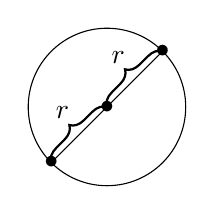
\begin{tikzpicture}
  \coordinate (C) at (0,0);
  \coordinate (P) at ({cos(45)}, {sin(45)});
  \coordinate (Q) at ({cos(225)}, {sin(225)});
  \def\r{1}

  \draw (Q) -- (P);
  \draw (C) circle (\r);

  \node at (P) {$\bullet$};
  \node at (C) {$\bullet$};
  \node at (Q) {$\bullet$};

  \draw[thick,decorate,decoration={brace,amplitude=5pt},yshift=2.5pt] (C) -- (P) node [midway,above,xshift=-6pt,yshift=2pt] {$r$};
  \draw[thick,decorate,decoration={brace,amplitude=5pt},yshift=2.5pt] (Q) -- (C) node [midway,above,xshift=-6pt,yshift=2pt] {$r$};
  
\end{tikzpicture}
